% Copyright 2004 by Till Tantau <tantau@users.sourceforge.net>.
%
% In principle, this file can be redistributed and/or modified under
% the terms of the GNU Public License, version 2.
%
% However, this file is supposed to be a template to be modified
% for your own needs. For this reason, if you use this file as a
% template and not specifically distribute it as part of a another
% package/program, I grant the extra permission to freely copy and
% modify this file as you see fit and even to delete this copyright
% notice. 

% \UseRawInputEncoding
\documentclass{beamer}

% There are many different themes available for Beamer. A comprehensive
% list with examples is given here:
% http://deic.uab.es/~iblanes/beamer_gallery/index_by_theme.html
% You can uncomment the themes below if you would like to use a different
% one:
%\usetheme{AnnArbor}
%\usetheme{Antibes}
%\usetheme{Bergen}
%\usetheme{Berkeley}
%\usetheme{Berlin}
%\usetheme{Boadilla}
%\usetheme{boxes}
%\usetheme{CambridgeUS}
%\usetheme{Copenhagen}
%\usetheme{Darmstadt}
%\usetheme{default}
%\usetheme{Frankfurt}
%\usetheme{Goettingen}
%\usetheme{Hannover}
%\usetheme{Ilmenau}
%\usetheme{JuanLesPins}
%\usetheme{Luebeck}
\usetheme{Madrid}
%\usetheme{Malmoe}
%\usetheme{Marburg}
%\usetheme{Montpellier}
%\usetheme{PaloAlto}
%\usetheme{Pittsburgh}
%\usetheme{Rochester}
%\usetheme{Singapore}
%\usetheme{Szeged}
%\usetheme{Warsaw}

\usepackage{pgfgantt}
\usepackage{todonotes}
\usepackage{media9}
\usepackage{fontawesome5}
\usepackage{subfigure}
\usepackage{booktabs,array}
\usepackage{tabulary}
\usepackage{caption}
\usepackage{graphicx}
\usepackage{siunitx}
\usepackage{arydshln}

\usepackage[ruled, vlined, linesnumbered]{algorithm2e} % For algorithms

\usepackage{amsmath} % For typesetting math

% Customize Warsaw color 
\setbeamercolor*{palette primary}{use=structure,fg=white,bg=red!50!black}
\setbeamercolor*{palette secondary}{use=structure,fg=white,bg=red!60!black}
\setbeamercolor*{palette tertiary}{use=structure,fg=white,bg=red!70!black}

% Customize Warsaw block title and background colors
\setbeamercolor{block title}{bg=red!50!black,fg=white}

\setbeamertemplate{bibliography item}{\insertbiblabel}  % insert bibliography numbers instead of symbol
\setbeamertemplate{caption}[numbered] % adds the figure or table number to the caption.


\title[HIL Plant Modeling]{Hardware-in-the-Loop Plant Modeling for Autonomous
  Vehicle}

% % A subtitle is optional and this may be deleted
\subtitle{Modeling, Simulation, and Testing}

\author[H.~Grady, N.~Nauman]{Hannah~Grady \and Nicholas~Nauman 
\linebreak Advisor:~Dr.~Suruz~Miah}
% - Give the names in the same order as the appear in the paper.
% - Use the \inst{?} command only if the authors have different
%   affiliation.

\institute[Bradley University] % (optional, but mostly needed)
{
  Department of Electrical and Computer Engineering\\
  Bradley University\\
  1501 W. Bradley Avenue\\
  Peoria, IL, 61625, USA
}
% - Use the \inst command only if there are several affiliations.
% - Keep it simple, no one is interested in your street address.

\date[October~7,~2021]{Thursday, October~7,~2021}

% - Either use conference name or its abbreviation.
% - Not really informative to the audience, more for people (including
%   yourself) who are reading the slides online

\logo{\hfill\href{http://www.bradley.edu}{
\includegraphics[width=0.75cm]{figs/logoBU1-Print}}}  % place logo in every page 


% \subject{Mobile Robot Localization}
% This is only inserted into the PDF information catalog. Can be left
% out. 

% If you have a file called "university-logo-filename.xxx", where xxx
% is a graphic format that can be processed by latex or pdflatex,
% resp., then you can add a logo as follows:

% \pgfdeclareimage[height=0.5cm]{university-logo}{university-logo-filename}
% \logo{\pgfuseimage{university-logo}}

% Delete this, if you do not want the table of contents to pop up at
% the beginning of each subsection:
\AtBeginSubsection[]
{
  \begin{frame}<beamer>{Outline}
    \tableofcontents[currentsection,currentsubsection]
  \end{frame}
}

% Delete this, if you do not want the table of contents to pop up at
% the beginning of each section:
\AtBeginSection[]
{
  \begin{frame}<beamer>{Outline}
    \tableofcontents[currentsection]
  \end{frame}
}

% Let's get started
\begin{document}

\begin{frame}
  \titlepage
\end{frame}

\begin{frame}{Outline} 
  \tableofcontents%[pausesections]
  % You might wish to add the option [pausesections]
\end{frame}

% Section and subsections will appear in the presentation overview
% and table of contents.
\section{Introduction}

\begin{frame}{Introduction}{}
    \begin{block}{Applications of Autonomous Vehicles}
    	\begin{itemize}
    		\item Autonomous vehicles are being developed by many companies for commercial and personal use
    		\item Modeling the steering system for autonomous vehicles is a challenging task
     		\item Models for autonomous vehicle subsystems must be very accurate due to safety factors
		\end{itemize}
    \end{block}
        \begin{figure}
			\centering
			\begin{minipage}[t]{0.4\textwidth}
				\centering
				\includegraphics[height=1.5cm]{figs/img/autonomousVehiclesAStuff}
				\caption{AutonomouStuff Vehicle Fleet\textsuperscript{a}}
				\label{fig:fleet}
			\end{minipage}
			\begin{minipage}[t]{0.4\textwidth}
				\centering
				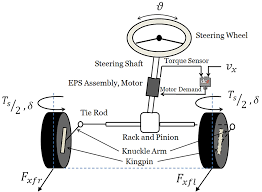
\includegraphics[height=1.5cm]{figs/img/autonomousVehiclesSteering}
				\caption{Autonomous Vehicle Steering System\textsuperscript{b}}
				\label{fig:steerSystem}
			\end{minipage}
        \end{figure}
    \begin{tiny}
		\textsuperscript{a}https://hexagonpositioning.com/pi-brands/autonomoustuff\\\textsuperscript{b}https://www.autonews.com/article/20181105/OEM10/181109921/delphi-s-pace-award-winning-e-steer-an-autonomous-vehicle-building-block
    \end{tiny}
\end{frame}

\begin{frame}{Problem Statement}
  \begin{block}{Problem Statement}
    \begin{large}
      Model vehicle subsystems for a Lexus platform.
 \begin{itemize}
          \item Steering Model
          \item Acceleration Model
          \item Brake Model
          \item Shift Model
          \item Speed Model
          \item Speed Control Model
        \end{itemize} 
    \end{large}
  \end{block}
  \pause
  \begin{block}{Proposed Solution}
    \begin{large}
      A potential solution is to develop conventional System Identification techniques for modeling subsystems using available raw data.  
    \end{large}
  \end{block}
\end{frame}

%----------------------------------

\section{Literature Review}

\begin{frame}{Literature Review}
  \begin{block}{Existing Solution}
 \begin{itemize}
        \item Use of System Identification Toolbox in Matlab to create models from data~\cite{Adnan2010}
	 \begin{itemize}
		    \tiny
		    		\item Offers a variety of model choices
				\item Needs a large amount of raw data to produce an accurate model
	\end{itemize}
	\item Third order ARMAX model creates models using traditional methods of analysis~\cite{Li1999}
	 \begin{itemize}
		    \tiny
		    		\item Allows the use of traditional analysis methods to create a model 
				\item More room for error during calculations
	\end{itemize}
	\item Steer-By-Wire method as a system model~\cite{Saruchi2015}
	 \begin{itemize}
		    \tiny
		    		\item Can model systems with small non-linearities 
				\item Mechanical components replaced by electrical components 
	\end{itemize}
\end{itemize}
  \end{block}
    % \begin{figure}[b]
    %     \centering
    %     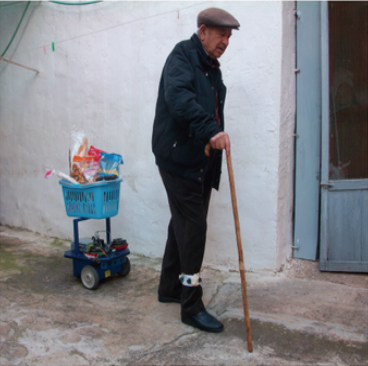
\includegraphics[width=0.45\textwidth]{figs/img/CompaRob}
    %     \caption{CompaRob}
    %     %\label{fig:sysBlockDiag}
    % \end{figure}
\end{frame}

%----------------------------------


\section{System Identification}

\begin{frame}{System Identification}
  \begin{block}{System Identification}
 \begin{itemize}
        \item System identification is the process of developing mathematical models for a dynamic system using the measurement of input and output signals of that system. The goal of the system identification methodology is to get an accurate estimation of the system response to any given input. Mathworks' MATLAB has the system identification toolbox, where a few existing examples demonstrate the working principle of this toolbox.
	\item 
	\item 
\end{itemize}
  \end{block}
\end{frame}

% \begin{frame}{Literature Review}
%   \begin{block}{Existing Solution}
%         Gated Recurrent Unit (GRU) network with LiDAR sensor and camera to map the customer~\cite{islam_lam_fukuda_kobayashi_kuno_2019}
%   \end{block}
%     \begin{figure}[b]
%         \centering
%         \includegraphics[width=0.40\textwidth]{figs/img/ShoppingSuportRobot}
%         \caption{Shopping Support Robot}
%         %\label{fig:sysBlockDiag}
%     \end{figure}
% \end{frame}

% %----------------------------------

% \begin{frame}{Literature Review}
%   \begin{block}{Existing Solution}
%     Arduino MEGA 2560, six ultrasonic sensors, two DC motors with Pulse Width Modulation (PWM), an Android Studio IDE device, and Bluetooth~\cite{Rawashdeh2017-Person}
%   \end{block}
%     \begin{figure}[b]
%         \centering
%         \includegraphics[width=0.50\textwidth]{figs/img/SmartCart}
%         \caption{Smart Cart Robot}
%         %\label{fig:sysBlockDiag}
%     \end{figure}
% \end{frame}

%----------------------------------

%\begin{frame}{Existing Solutions}
%  \begin{block}{Problems}
%    \begin{itemize}
%      \item Require line-of-sight between robot and user
%      \item Some require costly dedicated image processing hardware
%    \end{itemize}
%  \end{block}
%  \pause
%  \begin{block}{Benefits of Proposed Solution}
%    \begin{itemize}
%      \item High level of accuracy 
%    \end{itemize}
%  \end{block}
%\end{frame}

% \begin{frame}{Literature Review}
%   \begin{block}{Challenges}
%     \begin{itemize}
%       \item Communication between the robot and the remote
%       \item Buffer distance between the robotic cart and the customer without using line of sight sensing
%     \end{itemize}
%   \end{block}
% \end{frame}

%----------------------------------

\section{System Requirements}
\begin{frame}
\tiny
	\begin{block}{System Inputs and Outputs}
		\begin{itemize}
			\tiny
		    \item Steering Model
		    \begin{itemize}
		    \tiny
		    		\item Torque Voltages
		    		\begin{itemize}
		    		\tiny
		    			\item Desired Steering Wheel Angle
		    			\item Actual Steering Wheel Angle
		    		\end{itemize}
		    \end{itemize}
		    \item Acceleration Model
		    \begin{itemize}
		    \tiny
		    		\item Acceleration Pedal Voltages
		    \end{itemize}
		    \item Brake Model
		    \begin{itemize}
		    \tiny
		    		\item Brake Pedal Pressure Voltages
		    		\item Brake Pedal Stroke Voltages 
		    		\item Brake Pedal On/Off Switch
		    \end{itemize}
		    \item Shift Model
		    \begin{itemize}
		    \tiny
		    		\item Desired Shift Gear
		    \end{itemize}
		    \item Speed Model
		    \begin{itemize}
		    \tiny
		    		\item Acceleration Pedal Position
		    		\item Brake Pedal Position
		    		\item Shifter Actual Gear
		    \end{itemize}
		    \item Speed Control Model
		    \begin{itemize}
		    \tiny
		    		\item Desired Vehicle Speed
		    \end{itemize}
		\end{itemize}
	\end{block}
\end{frame}
\begin{frame}			
	\begin{figure}
		\includegraphics[width=10cm]{figs/inkscape/steeringModelArchitecture}
		\caption{Block Diagram of Steering Subsystem}
		\label{fig:steeringModel}
	\end{figure}
\end{frame}

\begin{frame}{System Requirements}
  \begin{block}{Specifications}
    \begin{itemize}
      	\item The plant model should have an accurate model of the six main subsystems
    		\item A hardware-in-loop (HIL) test bench can be developed from the plant models of the subsystems
    		\item The steering model can handle very small steering angles
    \end{itemize}
  \end{block}
\end{frame}

%--------------------------------

\section{System Architecture}

\begin{frame}{System Architecture}
  \begin{block}{}
 \begin{itemize}
        \item 
	\item 
	\item 
\end{itemize}
  \end{block}
\end{frame}

%----------------------------------

\section{Preliminary Work}

\begin{frame}{Preliminary Work}
  \begin{block}{Preliminary Work}
 \begin{itemize}
        \item Documentation on MATLAB's System Identification Toolbox and tutorials
        \item Literature Review 
        \item Data Collection for steering, braking and acceleration subsystems
\end{itemize}
  \end{block}
  \begin {block}{Modeling}
  \begin{itemize}
  	\item All modeling of vehicle subsystems will be done using MATLAB's System Identification Toolbox feature. The subsystems can be grouped into four different categories: Single-Input-Single-Output, Multiple-Input-Multiple-Output, Single-Input-Multiple-Output, and Multiple-Input-Single-Output. 
  	\end{itemize}
  	\end{block}
\end{frame}

%----------------------------------
\section{Simulation Results}

\begin{frame}{Simulation Results}
  \begin{block}{}
 \begin{itemize}
        \item 
	\item 
	\item 
\end{itemize}
  \end{block}
\end{frame}

%----------------------------------
\section{Parts List}

\begin{frame}{Parts List}
  \begin{block}{Software and Hardware}
 \begin{itemize}
        \item Software
        \begin{itemize}
        \small
        \item MATLAB's System Identification Toolbox
        \item Vector CANAlyzer
        \end{itemize}
	\item Hardware
	\begin{itemize}
	\small
	\item Laptop
	\item PAC Mod
	\item CAN Case 
	\item CAN Bus
	\end{itemize}
\end{itemize}
  \end{block}
\end{frame}

%----------------------------------
\section{Timeline and Milestones}

\begin{frame}{Timeline and Milestones}
  \begin{block}{Milestones}
 \begin{itemize}
        \item Model steering subsystem 
	\item Test subsystem models with HIL system 
	\item Final report and presentation 
\end{itemize}
  \end{block}
\end{frame}

%----------------------------------
\section{Timeline and Milestones}

\begin{frame}{Timeline and Milestones}

\end{frame}

%----------------------------------

\begin{frame}{Other Considerations}
  \begin{block}{Factors}
  	\begin{small}
      \begin{itemize}
        \item Public Health: Autonomous vehicles can make roads safer, which can prevent accidents
and driving fatalities and injuries. As a result, people will be able to live longer and
healthier lives. By creating accurate models, we will help advance the development of
autonomous vehicles and make this a reality.
		\item Public Safety: This is a relevant concern, because the real world implementations of inaccurate models could be disastrous since it is a self-driving vehicle. We will address this by creating a rigorous test plan for our models.
		\item Public Welfare: This factor is somewhat related to public safety and health in that we need to make sure that these vehicles are safe for people to use. How we will help
ensure this in our project is the same as how we will ensure public safety, by making sure we throughly test our models.
		\item Global Factors: 
		\item Cultural Factors: 
		\item Social Factors: 
		\item Environmental Factors: 
		\item Business Factors: 
		\item Economic Factors: 
      \end{itemize}
     \end{small}
  \end{block}
\end{frame}

%----------------------------------

\section{Concluding Remarks}
\begin{frame}{Concluding Remarks}
  \begin{block}{Project goals}
    \begin{LARGE}
      \begin{itemize}
        \item Develop models of an autonomous vehicle's subsystems
        \begin{itemize}
          \item Steering Model
          \item Acceleration Model
          \item Brake Model
          \item Shift Model
          \item Speed Model
          \item Speed Control Model
        \end{itemize}
      \end{itemize}
    \end{LARGE}
  \end{block}
  \begin{block}{Anticipated Challenges}
    \begin{itemize}
      \item Achieving an acceptable accuracy and reliability for each model due to its nonlinearities over small changes
    \end{itemize}
  \end{block}
\end{frame}

%----------------------------------

\section{References}

%\begin{frame}{References}
%  \bibliographystyle{IEEEtran}
%   \begin{itemize}
%     \item N. Rawashdeh, R. Haddad, O. Jadallah, and A. To’ma, “A person-following
% robotic cart controlled via a smartphone application: design and evaluation,”
% 09 2017, pp. 1–5.
%     \item M. M. Islam, A. Lam, H. Fukuda, Y. Kobayashi, and Y. Kuno, “An intelligent
% shopping support robot: understanding shopping behavior from 2d skeleton data using gru network,” ROBOMECH Journal, vol. 6, no. 1, 2019.
%     \item J. Sales, J. Marti, R. Marin Prades, E. Cervera, and P. Sanz, “Comparob: The
% shopping cart assistance robot,” International Journal of Distributed Sensor Networks, vol. 2016, pp. 1–15, 02 2016.
%     \item M. S. Miah, J. Knoll, and K. Hevrdejs, “Intelligent range-only mapping and navigation for mobile robots,” IEEE Transactions on Industrial Informatics, vol. 14, no. 3, pp. 1164–1174, 2018.
%     \item D. Li and S. Lane, “A novel and versatile parabolic reflector that significantly
% improves wi-fi reception at different distances and angles,” 2013.
  
%   \end{itemize}


% \end{frame}

%----------------------------------

\begin{frame}{References}

  \bibliographystyle{IEEEtran}
  \bibliography{bib/references.bib}

%\begin{itemize}
%\item
%@INPROCEEDINGS{Donjaroennon2021,
%  author={Donjaroennon, Natthapon and Nuchkum, Suphatchakan and Leeton, Uthen},
%  booktitle={2021 9th International Electrical Engineering Congress (iEECON)}, 
%  title={Mathematical model construction of DC Motor by closed-loop system Identification technique Using Matlab/Simulink}, 
%  year={2021},
%  volume={},
%  number={},
%  pages={289-292},
%  doi={10.1109/iEECON51072.2021.9440305}}
%\end{itemize}
% 	\begin{itemize}
% 		\item T. Xie, H. Jiang, X. Zhao, and C. Zhang, “A wi-fi-based wireless indoor position sensing system with multipath interference mitigation,” Sep 2019. [Online].
% Available: https://www.ncbi.nlm.nih.gov/pmc/articles/PMC6767237/
% 		\item A. M. Ladd, K. E. Bekris, A. Rudys, L. E. Kavraki, and D. S. Wallach, “Robotics-
% based location sensing using wireless ethernet,” Wireless Networks, vol. 11, no. 1-2, p. 189–204, 2005.
% 		\item M. Lindhe, K. Johansson, and A. Bicchi, “An experimental study of exploiting multipath fading for robot communications,” Robotics: Science and Systems III, 2007.
% 		\item M. Lindhe and K. Johansson, “Using robot mobility to exploit multipath fading,”Wireless Communications, IEEE, vol. 16, pp. 30 – 37, 03 2009.
% 	\end{itemize}

\end{frame}


\end{document}



%%% Local Variables:
%%% mode: latex
%%% TeX-master: t
%%% End:
